\section{Benchmark}\label{sec:benchmark}

In this section, we study a wide array of benchmarks.

\subsection{Block Update Comparison}\label{ssec:benchmark:pgd-newton}

In this section, we compare the algorithms presented 
in~\Cref{ssec:pgd,ssec:newton,ssec:newton-abs}
that solve the block update~(\ref{eq:bcd:block-update}).
Recall the objective to solve is
\begin{align*}
    \minimize_{\beta \in \R^p}
    \frac{1}{2} \beta^\top \Sigma \beta
    - v^\top \beta
    + \lambda \norm{\beta}_2
\end{align*}

\Cref{fig:bench:newton-compare} shows a set of comparisons
Newton, Brent, and Newton-ABS
(see~\Cref{ssec:newton,ssec:newton-abs}).
Although we also ran ISTA, FISTA, and FISTA with adaptive restart (FISTA-ADA)
(see~\Cref{ssec:pgd}), they failed to converge, so we omit their benchmark results.
All Newton methods properly converged.
For all scenarios, the diagonal of $\Sigma$ was generated uniformly from $[0, 1]$.
In addition,
\begin{enumerate}
    \item[(b)] \textbf{Almost PSD:} 1\% of the entries were regenerated uniformly from $[\num{1e-14}, \num{1e-8}]$.
    \item[(c)] \textbf{Very PSD:} 20\% of the entries were set exactly to zero and 10\% were regenerated from $[\num{1e-14}, \num{1e-8}]$.
\end{enumerate}
The vector $v$ was generated from $\Normal\pr{0, \Sigma}$.
Figures (a) to (c) used $\lambda=\num{1e-1}$ while (d) used $\lambda=\num{1e-4}$.
Both Newton-ABS and Brent methods are asymptotically faster than Newton,
however, Brent has the poorest performance for small to moderate $p$ ($\leq 100$).
Although, Brent performs slightly better than Newton-ABS when $D$ is positive definite,
we see that Newton-ABS is faster than Brent uniformly over $p$ when $D$ is PSD
by a larger margin.
Newton-ABS is up to 7 times faster than Newton and up to 4 times faster than Brent.
Given the robustness of Newton-ABS in speed and convergence across the different configurations,
we expect significant improvement to the overall optimizer using Newton-ABS.

\begin{figure}[t]
    \centering 
    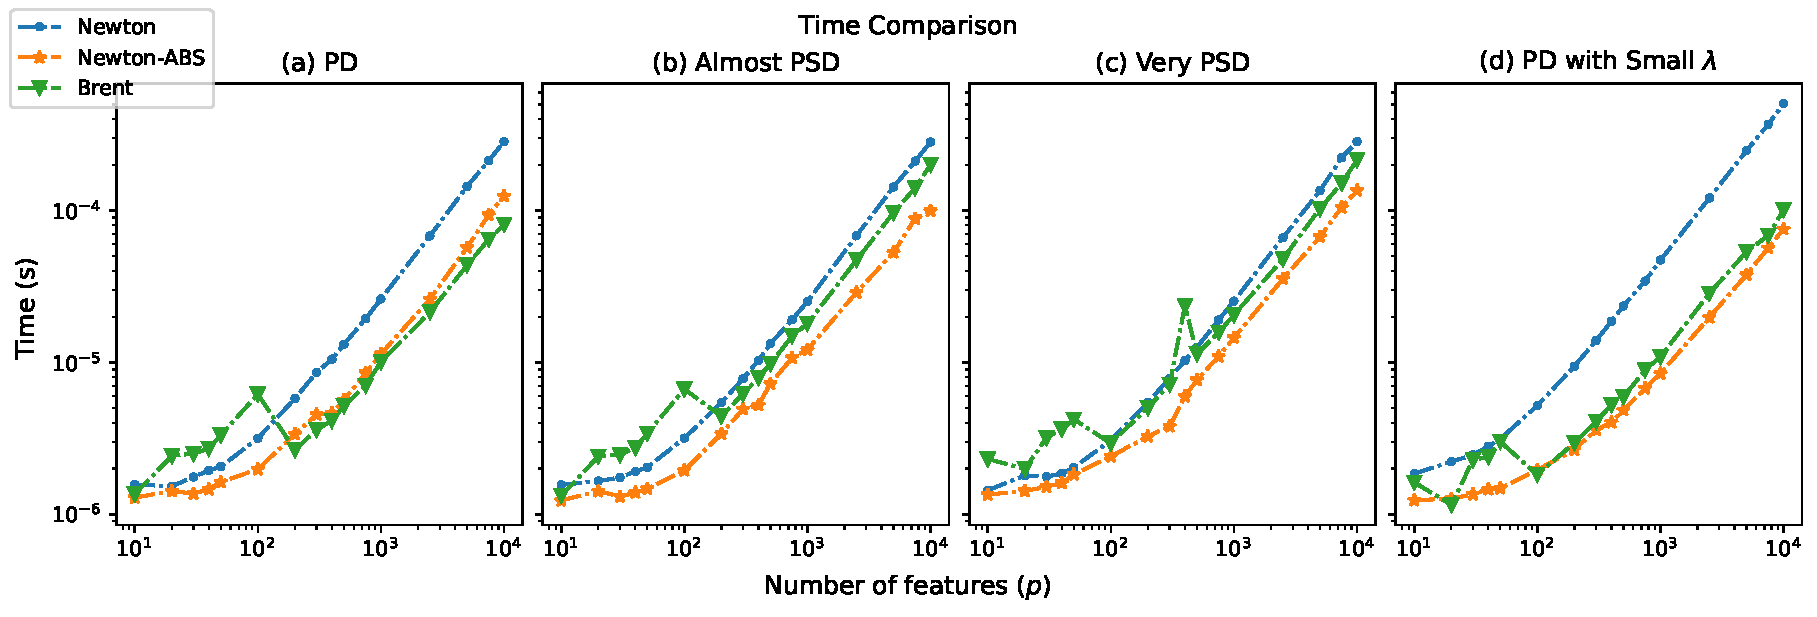
\includegraphics[width=\textwidth]{figures/newton_compare.pdf}
    \caption{Plot of runtimes for Newton, Newton-ABS, and Brent's Method
    for various input configurations.
    Figures (a) to (c) modifies the singularity of $D$ from positive definite to positive semi-definite.
    Figure (d) changes the regularization level to a smaller value.
    Overall, Newton-ABS is generally faster than Newton and Brent.
    Newton-ABS is up to 7 times faster than Newton and up to 4 times faster than Brent.
    }
    \label{fig:bench:newton-compare}
\end{figure}

\subsection{Benchmark against Other Packages}\label{ssec:benchmark:packages}

\begin{figure}[t]
    \centering 
    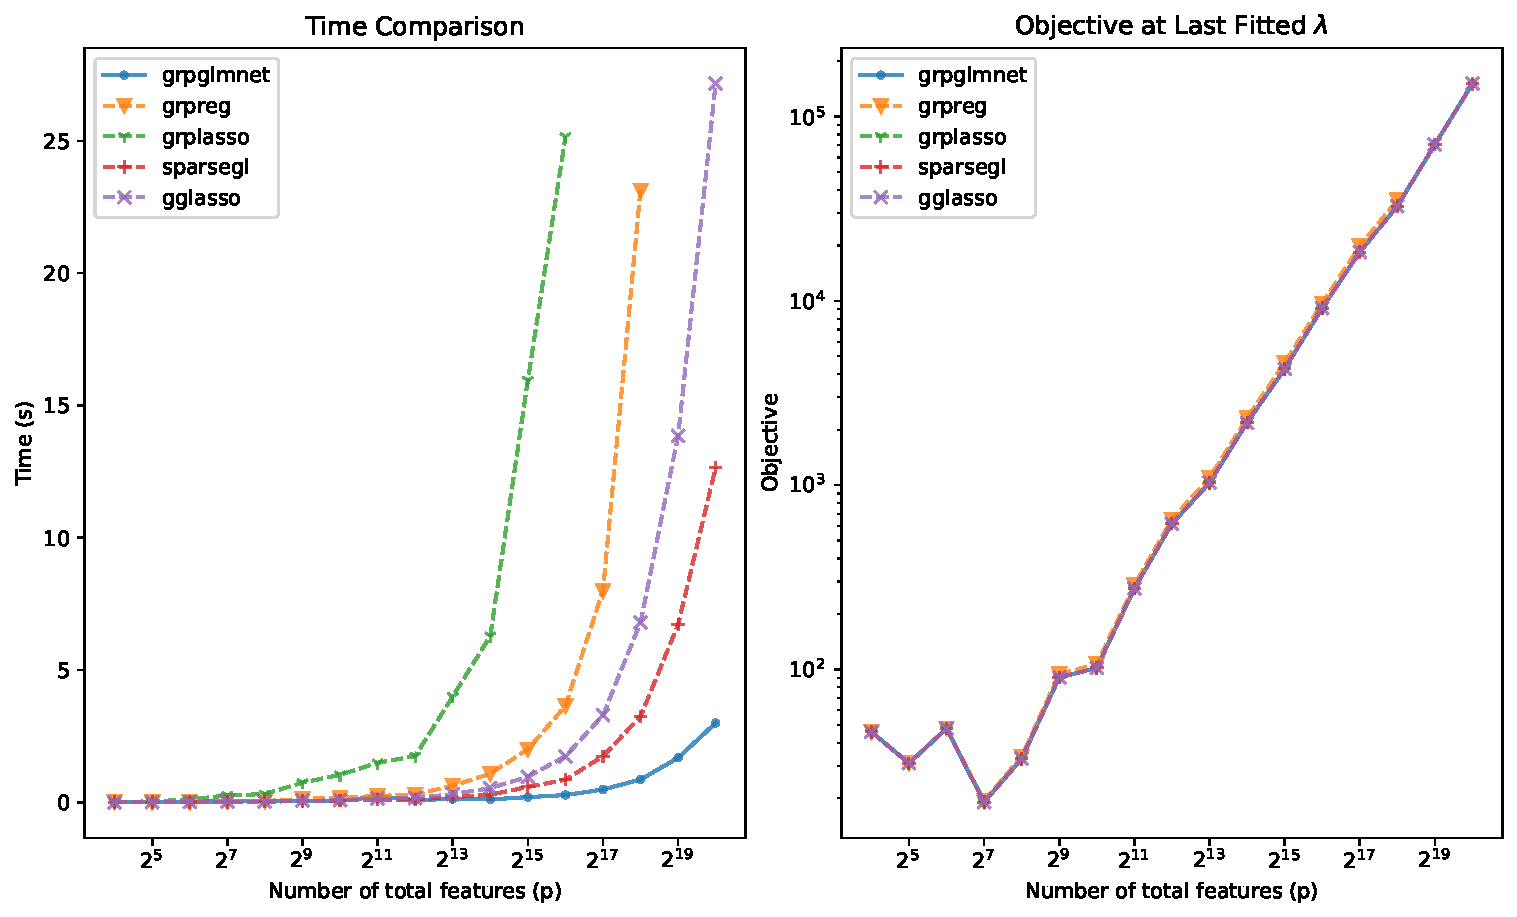
\includegraphics[width=\textwidth]{figures/package_comparison.pdf}
    \caption{Plot of runtimes and objective values for our package against other packages.
    The left plot shows that all packages perform well for small values of $p$,
    however, we quickly see a noticeable difference as $p$ grows.
    All packages converged as shown on the right plot.
    }
    \label{fig:bench:packages}
\end{figure}

\Cref{fig:bench:packages} shows a comparison of our package\todojames{name?}
against other packages: \texttt{grpreg}, \texttt{grplasso}, \texttt{sparsegl}, and \texttt{gglasso}.
We generate $X \in \R^{n \times p}$ where $n = 100$ and $p \in \set{2^4, \ldots, 2^{20}}$
and each entry is drawn from $\Normal(0,1)$.
The true coefficient vector $\beta$ is generated from $\Unif(-1,1)$ with 95\% of the entries
set to zero randomly.
Finally, we generate $y$ from the linear model: $y = X \beta + \epsilon$ where $\epsilon \sim \Normal(0, I_n)$.
The groups are generated with a group size of 10 
by grouping consecutive coefficients with the possible exception
of the last group, which may contain any remaining coefficients.
We center both $X$ and $y$, and scale each column of $X$ such that its norm is 1.
The regularization path was kept the same across all packages for each data generation.
\texttt{grpreg} produced an error for $p \geq 2^{19}$
and \texttt{grplasso} took too long for large $p$, so we omit these results.
All packages converged, however, \texttt{grpreg} generally had a larger objective.
We clearly see that our package\todojames{name?}
performs significantly faster, especially with large $p$.
With $p = 2^{20}$ (approximately 1 million features), our package\todojames{name?}
fits a path of about 55 regularization values in \textbf{3 seconds},
while the next fastest package, \texttt{sparsegl}, runs in \textbf{13 seconds},
and the next fastest, \texttt{gglasso}, runs in \textbf{27 seconds}.

